%& -shell-escape

\documentclass[letter]{article}

\usepackage[utf8]{inputenc}
\usepackage{amsmath}
\usepackage[round]{natbib}
\usepackage{graphicx}
\usepackage{todonotes}
\usepackage{colonequals}
\usepackage{mathtools}
\usepackage[running]{lineno}
\usepackage{setspace}
\usepackage[nostamp]{draftwatermark}
\usepackage[ruled]{algorithm2e}
\usepackage{python}
%\usepackage{subcaption}
\usepackage{subfig}
\usepackage{rotating}

\linenumbers
\onehalfspacing

\DeclareMathOperator*{\argmin}{arg\,min}
\DeclareMathOperator*{\argmax}{arg\,max}

\title{Restoring credibility to distributed wood supply planning: a case study}

\author{
  Gregory Paradis\\
  Luc LeBel\\
  Sophie D'Amours\\
  Mathieu Bouchard
}

\begin{document}
\maketitle

\begin{abstract}
  Foo. 
\end{abstract}


%\doublespacing
\section{Introduction}
\label{sec:introduction}

The concept of sustainable forest management (SFM) has long been a central theme of Crown (public) forest policy in Canada \citep{ccfm2008vision}. In concrete terms, sustainable forest management policy is implemented via silviculture treatments, noteably harvesting treatments. According the the \emph{Critian and Indicators of Sustainable Forest Management in Canada} \citep{ccfm2006criteria}, sustainability of harvest level is deemed to be sustainable if it is below annual allowable cut (AAC) level. 

The term \emph{wood supply planning} describes the process by which AAC is determined. In practice this typically amounts to solving a linear programming (LP) optimization model, which maximizes AAC subject to even-flow constraints \citep{gunn2007models}. Provincial government authorities allocate timber licences (TL) to industrial fibre consumers. These TLs set (species-wise) upper bounds on periodic harvest volume, however there is typically no policy requirement to set a matching lower bounds. 

%This implies that 

%Wood supply planning plays an important role in sustainable forest management. This is particularly true on Crown (public) forest land in Canada, where government steward manage the forest resource on behalf of the Canadian people. 

The timber licences are typically valid for a pre-determined period (e.g., 5 years), after which the may be renewed, subject to re-evaluation of species-wise AAC. Figures \ref{fig:aac} and \ref{fig:jointdist}(a) show species-wise Canadian AAC data from 1990 to 2012. Although there is some fluctuation over time, total national AAC has been relatively stable during this period.

For a variety of economic and logistic reasons, some portions of the AAC are not attractive the the timber licencees and are not harvested. Figures \ref{fig:aac_consumption} and \ref{fig:jointdist}(b) show species-wise proportion of Canadian AAC consumed from 1990 to 2012. On average, 80\% of softwood AAC is consumed, versus 45\% of hardwood AAC, indicating a clear industrial preference for softwood. Consumption rates for both species groups show similar variability. Softwood AAC consumption appears to be following a slight downward trend, whereas hardwood AAC consumption appears to be on the rise. 

\begin{figure}[h]
  \centering
  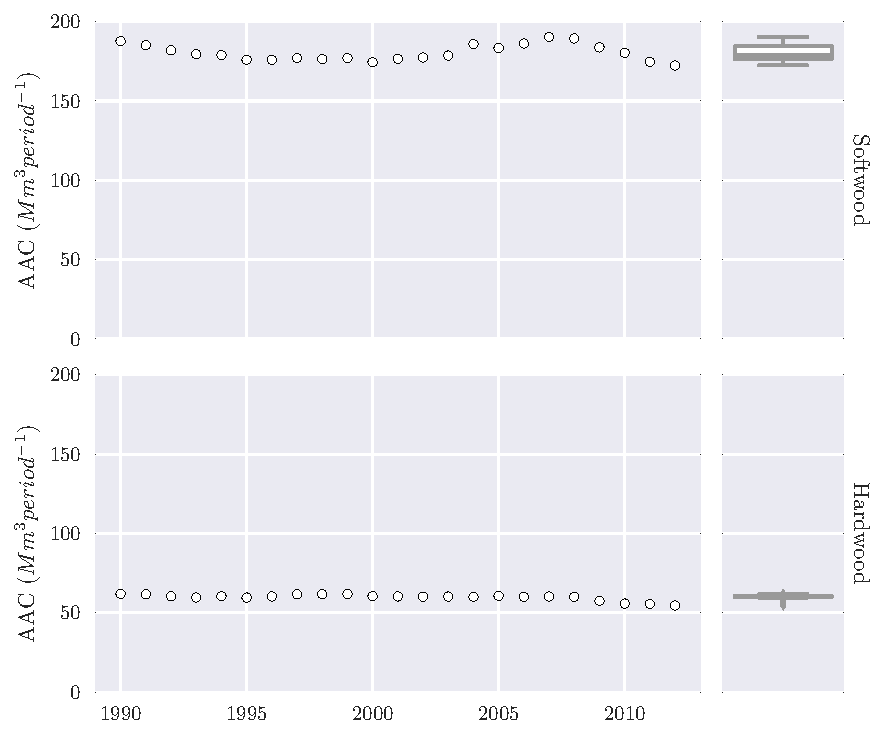
\includegraphics[width=\textwidth]{images/aac}
  \caption{Species-wise AAC consumption for period 1990 to 2012}
  \label{fig:aac}
\end{figure}

\begin{figure}[h]
  \centering
  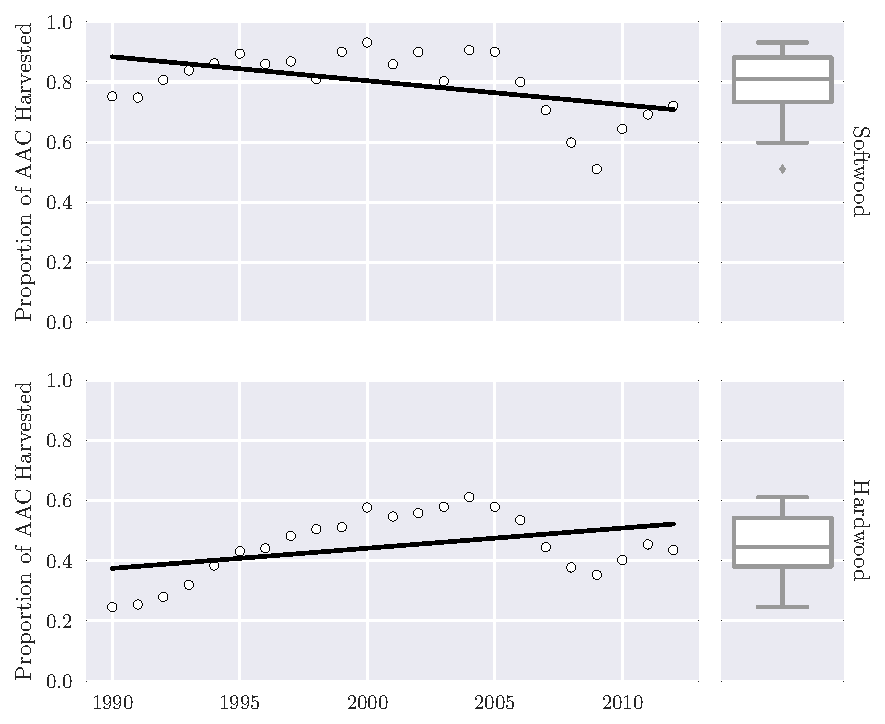
\includegraphics[width=\textwidth]{images/aac_consumption}
  \caption{Species-wise AAC consumption for period 1990 to 2012}
  \label{fig:aac_consumption}
\end{figure}

\begin{figure}[t]
    \centering
    \subfloat[AAC]{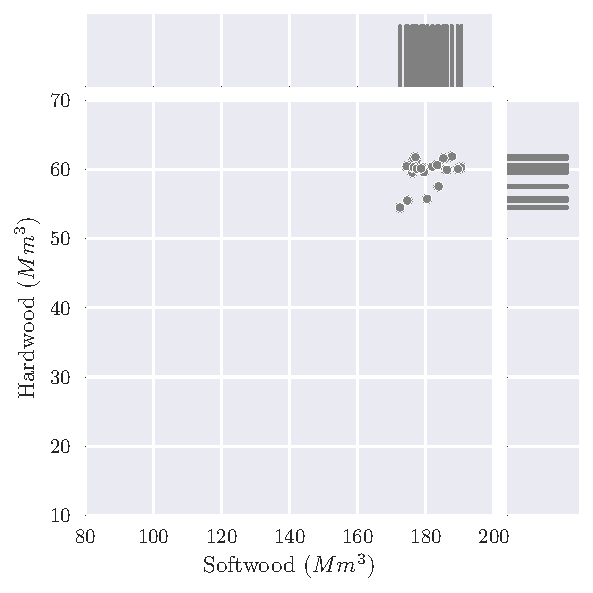
\includegraphics[width=0.5\textwidth]{images/aac_jointplot}}
    \subfloat[Fibre consumption]{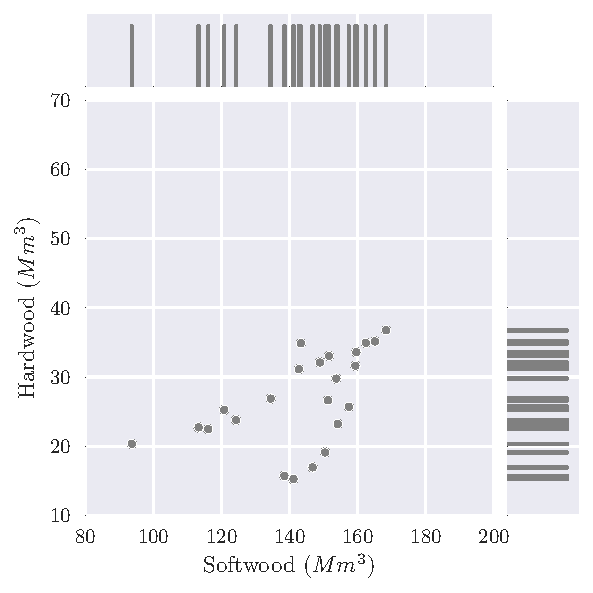
\includegraphics[width=0.5\textwidth]{images/harvest_jointplot}}
  \caption{Species-wise joint distributions of AAC and harvest volume for period 1990 to 2012}
  \label{fig:jointdist}
\end{figure}

% \begin{figure}[t]
%     \centering
%     \begin{subfigure}[t]{0.5\textwidth}
%         \centering
%         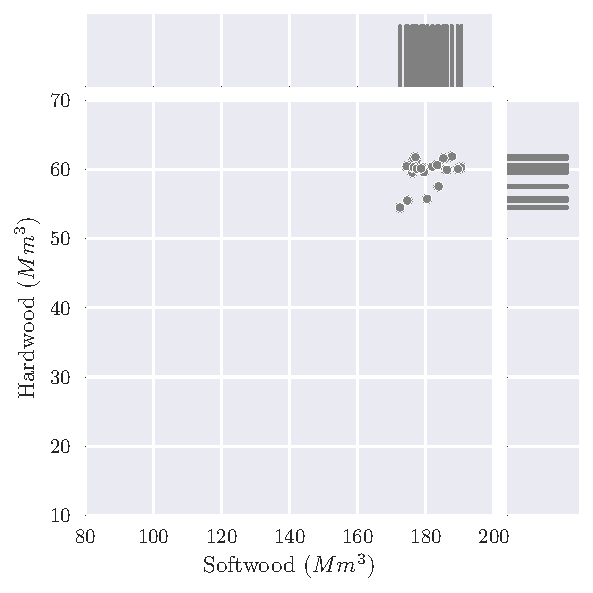
\includegraphics[height=\textwidth]{images/aac_jointplot}
%         \caption{AAC}
%     \end{subfigure}%
%     \begin{subfigure}[t]{0.5\textwidth}
%         \centering
%         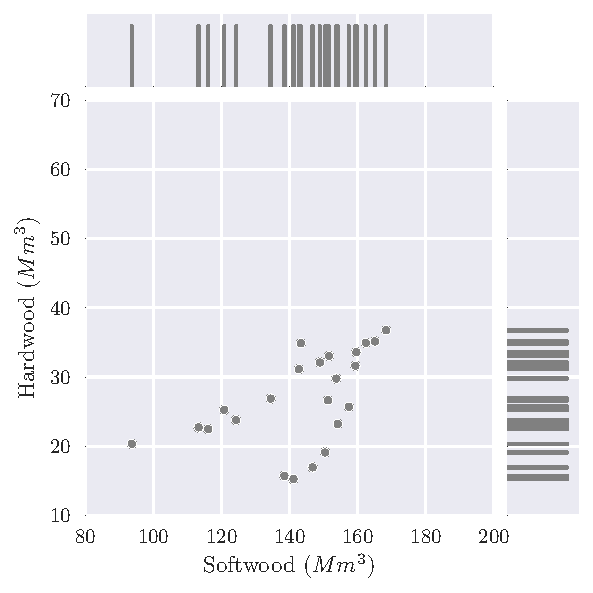
\includegraphics[height=\textwidth]{images/harvest_jointplot}
%         \caption{Harvest Volume}
%     \end{subfigure}
%   \caption{Species-wise joint distributions of AAC and harvest volume for period 1990 to 2012}
%   \label{fig:jointdist}
% \end{figure}


The data show a species-skewed negative consumption bias, relative to AAC, which is related to the infinite-demand assumption implicitly embedded in the classic wood supply optimization model formulation. 
%which is the \emph{de facto} standard tool used by government authorities to determine AAC on Crown land. 
\citet{paradis2013risk} estimate the impact of this bias, using a sequence of 30 two-phase rolling-horizon planning cycles\footnote{The first phase simulates determination of AAC by government officials, and the second phase simulates consumption of a profit-maximizing subset of available fibre by forest products industry firms.}, and show that consuming a species-skewed subset of AAC can induce future wood supply failures under certain conditions. They conclude that the wood supply planning process currently in place on Crown land in Canada does not provide credible assurance of long-term sustainability of the wood supply. Given the pervasiveness of the species-skewed negative consumption bias, the classic wood supply optimization model formulation is clearly not a rational basis for the implementation of a sustainable forest management policy. 

\citet{paradis2014bilevel} address this problem by developing a novel bilevel extension of the classic wood supply optimization model formulation. Through explicitly anticipating short-term industrial fibre consumption behaviour, the bilevel wood supply model formulation was shown to reduce the magnitude and species-skewedness of the AAC consumption bias. \citet{paradis2013risk} conjecture that closing the gap between AAC and industrial fibre consumption should improve the credibility of long-term wood supply projections.

The objectives of this study are to (a) compare the long-term performance of the classic and bilevel wood supply optimization model formulations, and (b) provide recommendations for improving the credibility of the wood supply planning process.


% Unrealistic assumptions regarding industrial fiber consumption behaviour are currently embedded into this \emph{classic} optimization model used to determine annual allowable cut (AAC). 
% These unrealistic assumptions are inducing biased distortions of the
% As a result, these models are failing to provide credible assurance of long-term sustainability of timber supply on public land.

% When fibre consumption is systematically lower than AAC,  the long-term planning process is unlikely to provide credible information regarding sustainability of the wood supply. 
% In practice, harvest levels are often lower than AAC if (a) aggregate timber demand is lower than AAC, (b) composition of harvested stands in AAC model is incoherent with timber demand, or (c) portions of projected AAC harvest volume are economically or operationally unattractive. 
% If left unresolved, this biased incoherence between planned and executed harvesting activity levels has been shown to destabilize the wood supply in certain cases \citep{paradis2013risk}. 

% \citet{paradis2014bilevel} present a bi-level extension of the classic wood supply model. Using a game-theoretic approach based on the principal-agent problem, they explicitly anticipate industrial fibre consumption behaviour within the wood supply planning model. Their extended model closes most of the gap between planned and executed harvesting activities. Potential long-term benefit of using this extended wood supply model formulation include improving credibility of the wood supply planning process, stabilizing fibre supply volume, and stabilizing value-creation potential. 


%\section{Background}
%\label{sec:background}

\section{Materials and Methods}

\subsection{Study Area}

The study area is a forest management unit (FMU 031-53) located in the boreal forest region of the province of Quebec, Canada. It covers an area of approximately 102 040 hectares. 
%The forest inventory data for this area was compiled into a number of management strata for the purposes of wood supply modeling.  
Approximately (88\%) of initial growing stock is from softwood species, with the remaining (12\%) of initial growning stock in hardwood species. 
Although some pure softwood stands are present, forest cover is dominated by mixed-wood stands containing different proportions of
hardwood mixed in with the softwood. See \citet{paradis2013risk} for a more detailed description of the study area.

\subsection{Simulation Framework}

We use the two-phase rolling-horizon simulation framework developed by \citet{paradis2013risk} as a testbed in which to compare the long-term performance classic and bilevel wood supply model formulations. This framework uses agency theory to model interaction between government wood supply planners (the \emph{principal} and industrial fibre consumers (the \emph{agent}.

% assumes that long-term AAC-maximizing wood supply planning is controlled by government planners (the \emph{principal}), and that short-term profit-maximizing fibre consumption is controlled by industry planners (the agent). 
The principal and the agent get to make their moves sequentially, in a two-phase game, repeated 30 times (simulating 5-year rolling-horizon re-planning cycles). The principal has the advantage of first move, which means he can set AAC to any level of his choosing. The simulation results presented here therefore show the cumulative result of 150 years of iterative replanning, under different combinations of principal and agent behaviour. 

\subsubsection{Wood Supply Model}

This study compares the performace of two wood supply model formulations. The classic wood supply model maximizes even-flow AAC, and is described in detail in \citet{paradis2013risk}. 

The bilevel formulation extends this model with a fibre-consumption-anticipation constraint. This sets output-wise uppers bounds on AAC, such that all harvest volume must be eminently consumable by an industrial network. This anticipation constraint is itself formulated as an optimization model (maximizing first-period agent profit), inducing the bi-level structure. The bi-level problem is much more difficult to solve than the original problem.  \citet{paradis2014bilevel} describe a novel method which can solve a special case of the bilevel model to global optimality, using computational effort comparable to that required to solve the classic model.

\subsubsection{Industrial Fibre Consumption Model}

We simulate industrial fibre consumption by simulating profit-maximizing behaviour of a network of business units, which we segregate into \emph{softwood} and \emph{hardwood} lines, each of which must be independently profitable. Our industrial data set was intentionally configured with a relatively small hardwood sawmill, whose processing capacity is approximately one-third of initial hardwood AAC. When combined with a clearcut-only policy and the relative abundance of mixed wood stands, the hardwood bottleneck indirectly limits softwood fibre consumption. 

See \citet{paradis2013risk} for a more detailed description of the test dataset and the iterative simulation framework used in the computational experiments.

\subsection{Scenarios}

We present six scenarios, showing impact of replacing the classic wood supply model with the bi-level wood supply model. Within any given scenario, simulation parameters for the industrial fibre consumption network\footnote{Mill capacities, costs, prices, client demand, etc.} are held constant for all 30 planning cycles. Table X summarizes the key simulation parameters for each scenario. 


Scenairo 1 simulates the \emph{status quo} behaviour for both principal and agent, and acts as a control scenario. At each planning cycle, the principal maximizes even-flow AAC (30-period horizon) using the classic wood supply model, then the agent maximizes first-period profits (1-period horizon) by consuming the optimal subset of the wood supply offered by the principal. The principal does not consider the agent's fibre consumption capacity when determining AAC. 

Scenario 2 presents a perfect-implementation bilevel scenario; rather than being allowed to re-plan harvesting on a one-period horizon, the agent is forced to exactly implement the first period of the principal's bilevel wood supply solution. This scenario shows the best-case performance of the bilevel model solution, and is equivalent to the principal controlling the entire wood procurement process from stump to mill gate.

Scenario 3 is the basic bilevel scenario. The principal uses the bilevel model to determine AAC, and the agent is allowed to replan harvesting on a one-period horizon, choosing the profit-maximizing subset of available wood supply. Due to the optimal formulation of the bilevel model and perfect anticipation of volume consumption, the agent always chooses to harvest the entire wood supply. However, the agent may select to harvest this volume from a different combination of forest types than what was prescribed in the first period of the principal's optimal solution. This reflects the distributed nature of forest management planning on Crown land in many jurisditions.

The contrast between scenario 1 and scenario 2 shows the sensitivity of long-term wood supply to deviations from the principal's optimal wood supply plan.

Scenarios 4 and 5 show the effect of reducing the wood supply allocated to the agent to 80\% and 60\% of AAC on long-term wood supply stability. Adjusting the AAC to allocation ratio is an indirect way to implement a buffer stock to protect against decreases in wood supply induced by agent harvest re-planning (i.e., compensation for the principal's incomplete control of the fibre procurement process).

Scenario 6 shows the effect of simulating centralized agent fibre procurement planning on long-term wood supply. For this scenario, we relax the agent's line-wise profitability contraint, and allow him to maximize total network profit. For this scenario, we allow any overflow fibre (hardwood, in our case) to be disposed of at a moderate unit cost. This allows the agent's softwood line to subsidize the disposal of excess hardwood from harvesting of mixedwood stands, thereby increasing the agent's total potential fibre consumption. This in turn relaxes the lower-level consumption constraints in the principal's bilevel model, thereby allowing him to increase the wood supply offer without compromising long-term sustainability. 

%Scenarios 2 through 6 replace the classic wood supply model with with bilevel model. These scenarios show the long-term cumulative impact of anticipating industrial fibre consumption behaviour withing the AAC-determination process. 

%Scenarios 1, 3, 4 and 5 simulate standard agent behaviour; the agent is allowed to select any available forest units for harvesting in the first period, subject to species-wise AAC upper-bound constraints. The agent harvests the entire wood supply for both species groups. This is expected behaviour, given that we simulate perfect anticipation of agent behaviour (i.e., we use the same optimization model formulation for both the agent-anticipation constraint embedded into the bilevel model, and for simulation of agent consumption behaviour in the second phase of the rolling-horison replanning simulation, as in \citet{paradis2014bilevel}. Note that although the the anticipation mechanism embedded into the bilevel model perfectly anticipate the \emph{volume} of fibre consumption, these may be harvested from different forest units than than the ones that make up the basis of the first period of principal's optimal wood supply solution. This reflects the distributed nature of forest management planning on Crown land.

%Scenario 2 forces the agent to exactly implement the principal's first-period optimal solution. This is an optimistic scenario, to illustrate the best-case performance of the bilevel model solution.




\section{Results}
\label{sec:results3}

Figures \ref{fig:scenarios} shows simulation results the six scenarios described in the previous section. For each scenario, Figure \ref{fig:scenarios}(a) plots species-wise AAC and fibre consumption for each of the 30 rolling-horizon re-planning cycles simulated. The same data are shown in Figure \ref{fig:scenarios}(b) using boxplots to illustrate the variability of period AAC and fibre consumption values across scenarios. The boxes encompass the inter-quartile range (IQR) with the median marked. The whiskers extend to 1.5 * IQR past the closest quartile; any observations outside this range are marked as outliers using a dot sybol.


\begin{sidewaysfigure}%
  \centering
  \subfloat[][]{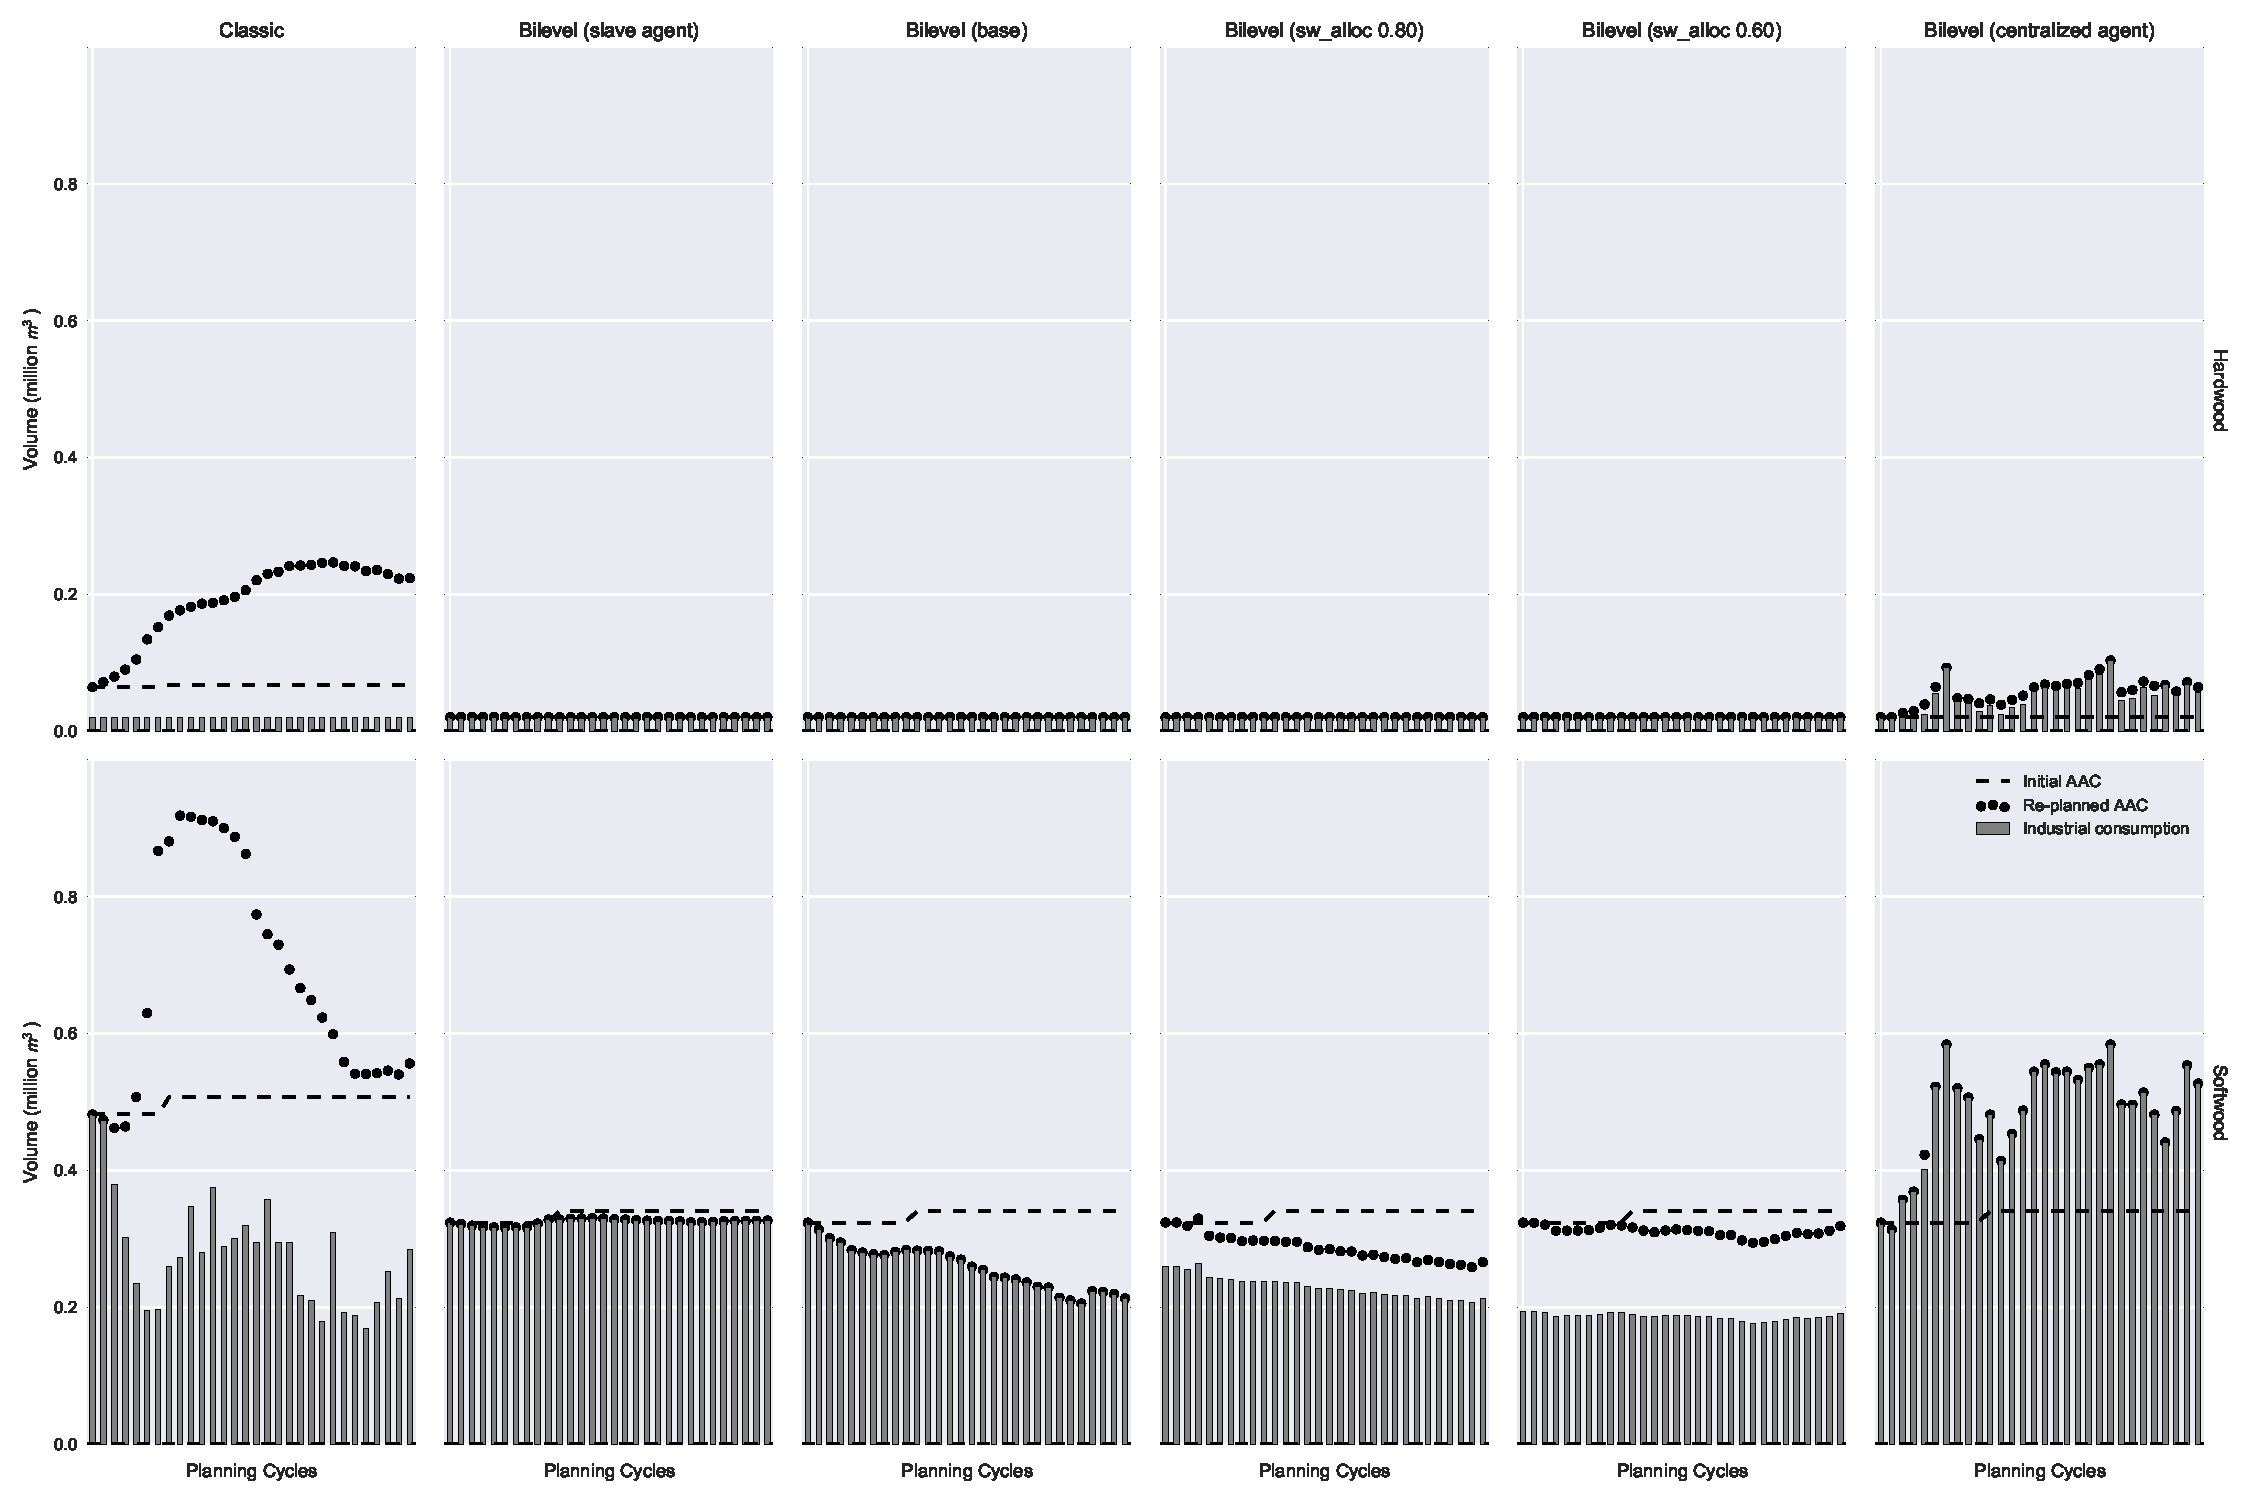
\includegraphics[width=\textwidth]{images/scenarios_timeseries}}%
  \caption{Species-wise AAC and fibre consumption for scenarios 1 to 6 (time series)}%
  \label{fig:scenarios}%
\end{sidewaysfigure}

\begin{sidewaysfigure}%
  \ContinuedFloat
  \centering
  \subfloat[][]{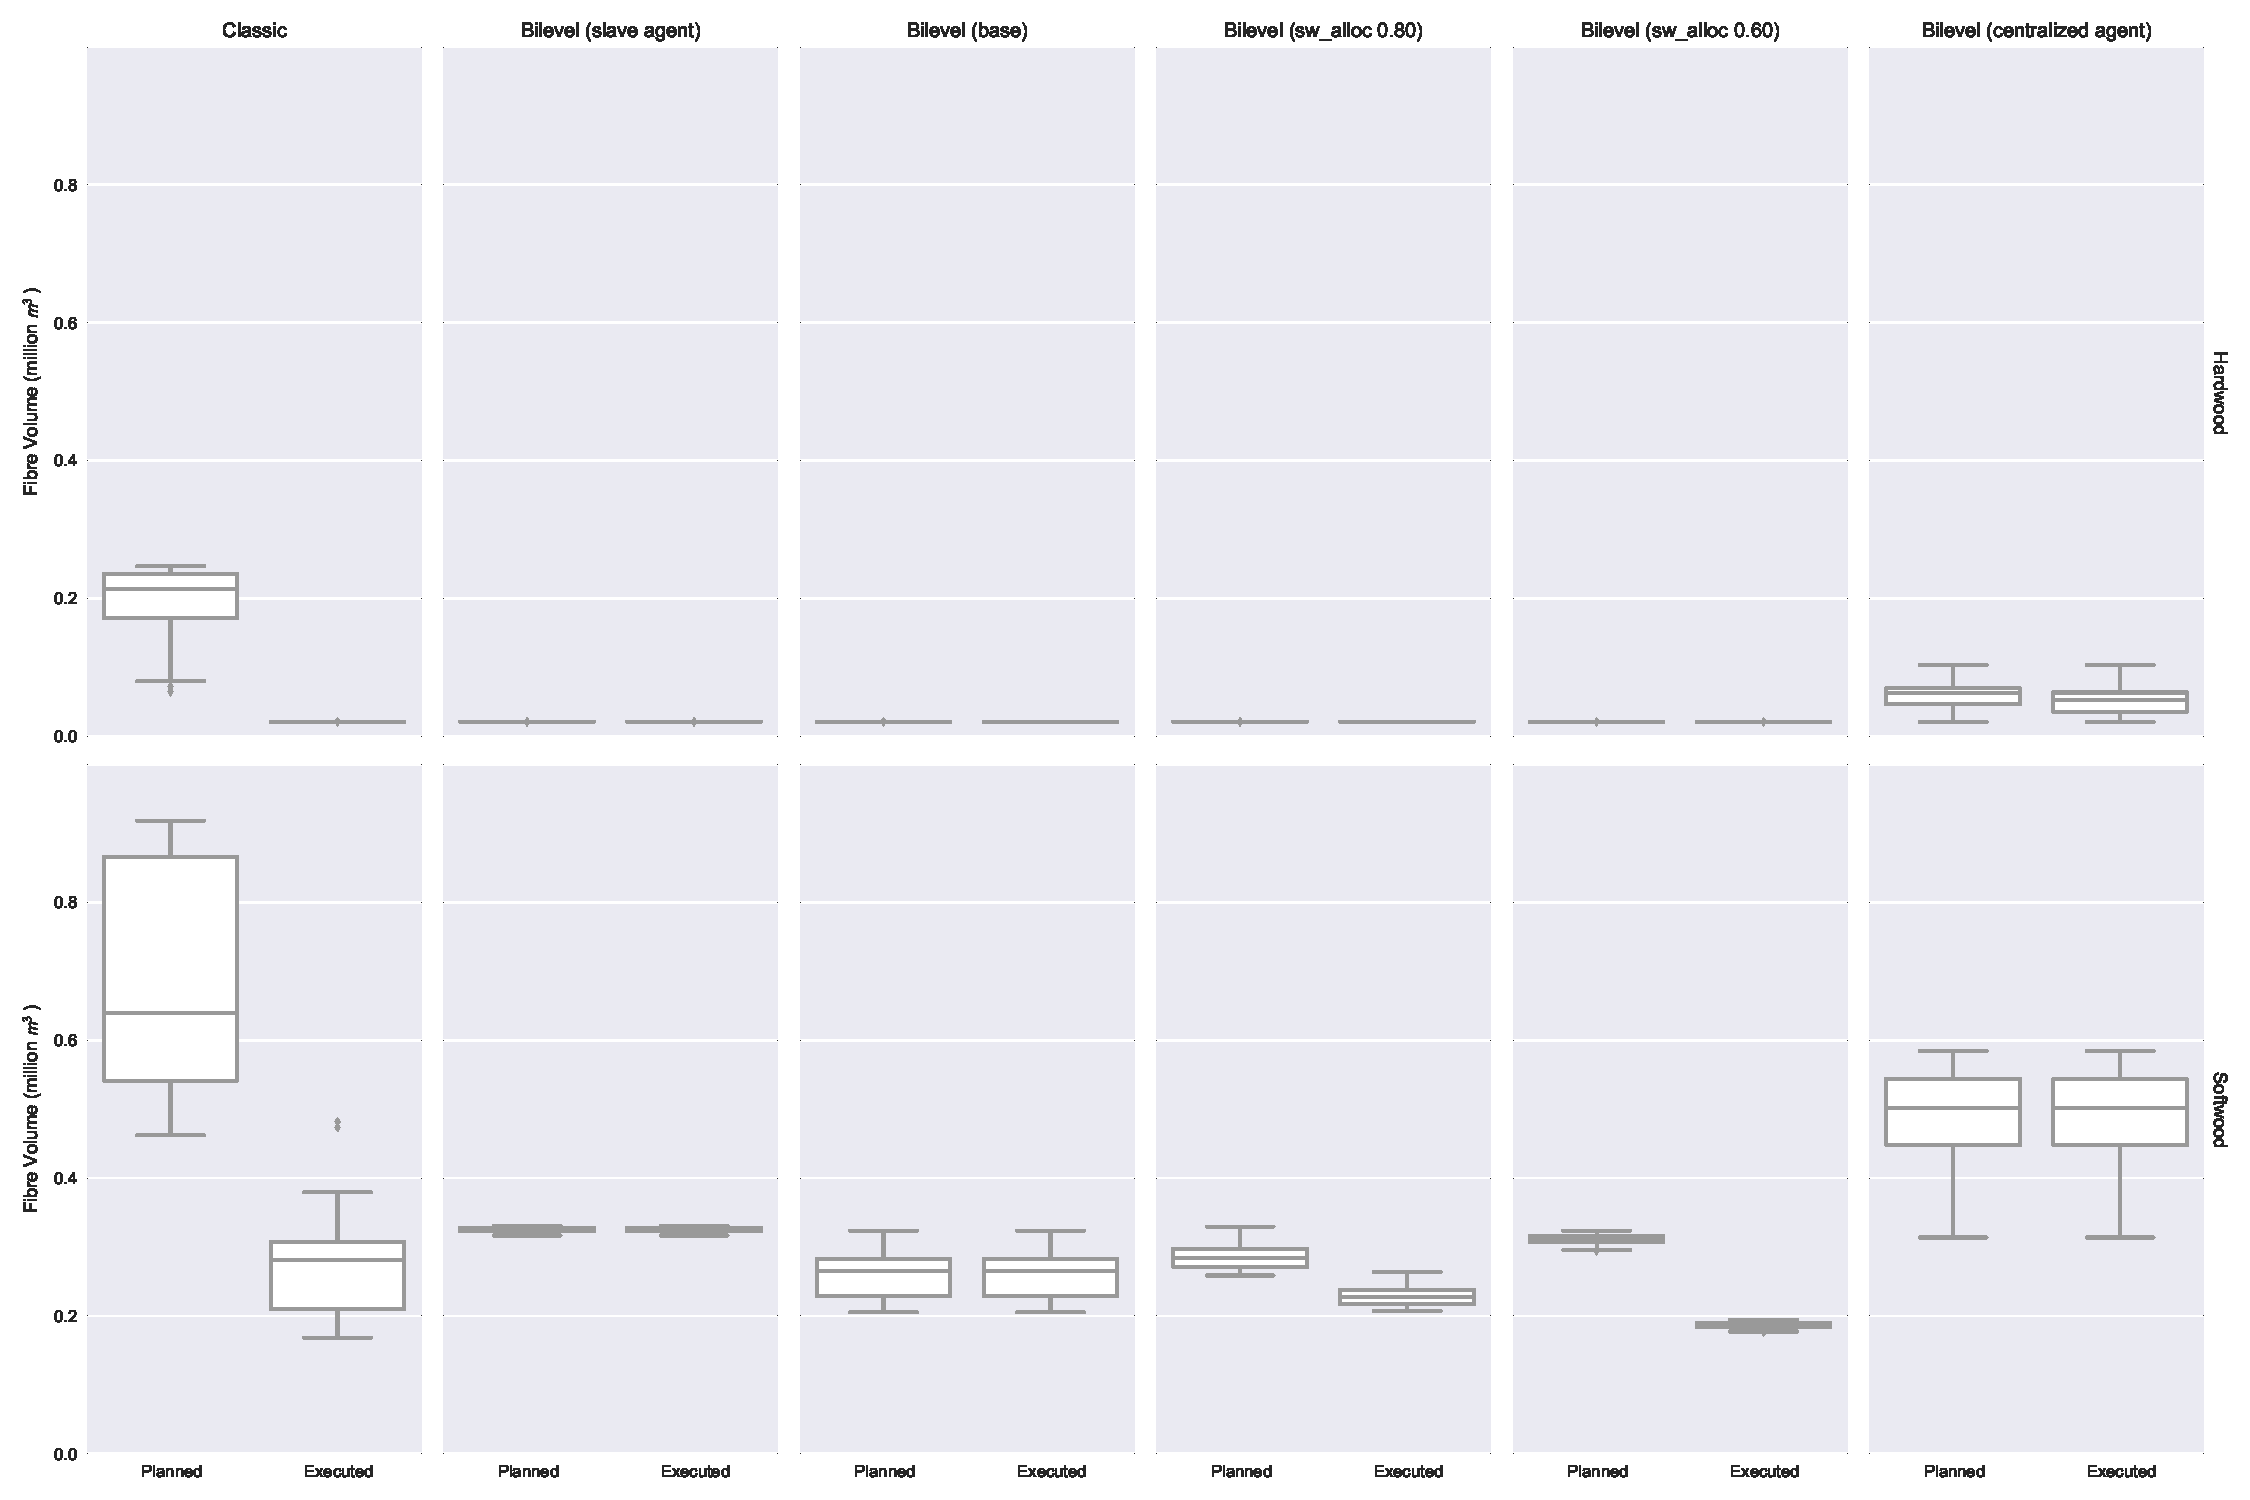
\includegraphics[width=\textwidth]{images/scenarios_boxplots}}%
  \caption{Species-wise AAC and fibre consumption for scenarios 1 to 6 (boxplots)}%
  %\label{fig:scenarios_boxplot}%
\end{sidewaysfigure}

%\begin{figure}%
%  \ContinuedFloat
%  \centering
%  \subfloat[][]{...figure code...}%
%  \caption[]{Species-wise AAC and fibre consumption for scenarios 1 to 6 (boxplots)}%
%  \label{fig:scenarios}%
%\end{figure}

\section{Discussion}

Scenario 1 shows the relative instability of the classic wood supply model. This is attributable to the species-skewed gap between AAC and fibre consumption volumes. Despite the harvest levels being systematically lower than AAC, the agent's preference for harvesting high-softwood-content stands gradually shifts the composition of the residual forest cover towards a higher hardwood content. \citet{paradis2013risk} use the term \emph{systematic drift effect} to describe this phenomenon.   

The principal uses the bilevel model to determine AAC for scenarios 2 through 6. By virtue of its formulation, the bilevel model completely eliminates the volume gap between AAC and fibre consumption. Note that we simulate perfect anticipation of agent fibre consumption \emph{volume}. For scenarios 3 through 6, we allow the agent to plan his own harvesting in the second phase of each planning cycle simulation; this explains the residual instability in long-term wood supply.

Scenario 2 forces the agent to harvest the exact forest units that form the basis of the first period of the principal's optimal bilevel solution. The purpose of this scenario is to show that wood supply tracks almost perfectly along the initial AAC solution (even after 30 rolling-horizon re-planning cycles) under best-case conditions (i.e., when the principal controls wood procurement planning execution all the way to the mill gate). In practice, the decoupling point between the principal and the agent is not typically located this far downstream; scenarios 3 through 6 simulate a more conventionnal decoupling point.

Scenario 3 shows vastly improved stability (hence credibility) of the softwood supply levels. Note the slight, but monotonic, downward trend of the softwood fibre supply. As discussed earlier, this shows that the bilevel model is sensitive to even slight deviations from the mix of forest units prescribed in the first period of the optimal solution. This type of sensitivity to deviations from the optimal solution is typical of deterministic optimization models, as optimal solutions are invariably located along the boundary of the feasible region; even the slightest deviations from the optimal solution (or in the constraint right-hand-sides) can induce problem infeasibility.

Scenarios 4 and 5 show the effect of reducing the proportion of AAC that is allocated to the agent, in an attempt to compensate for the residual drift seem in scenario 2. Reducing the allocation proportion is an indirect way for the principal to induce a buffer stock in the standing timber inventory. This tends to move the agent's solution away from the feasible boundary of the principal's solution space, thereby improving the robustness of the distributed wood supply planning process. Scenario 4 shows a marked reducting in drift compared with scenario 3. Residual drift is virtually eliminated in scenario 5, but at the expense of 40\% of the maximum potential (bilevel) sustainable wood supply. 

Intuitively, foregoing 40\% of the potential wood supply seems like a high price to pay to eliminate the residual drift in a bilevel modelling context. A more direct management approach to maintaining a buffer stock in teh standing timber inventory, as described in \citet{raulier2014increasing}, may be a more efficient approach to reducing the residual drift in a distributed wood supply planning context. 

By stabilising the long-term wood supply, scenario 5 \emph{does} succeed in restoring credibility, albeit at a relatively high cost in terms of the magnitude of the wood supply. Scenario 5 makes no optimistic assumptions regarding agent behaviour (in contrast with scenarios 2 and 6). Also, it is the only scenario in this series to respect the even-flow pattern prescribed by the wood supply model constraints.  Assuming that the even-flow constraints are valid and necessary (although not sufficient) conditions for sustainbility of the forest management plan\footnote{There has been considerable debate in the literature over the validity and necessity of including even-flow or non-declining yield constraints in wood supply optimization models. Nonetheless, one or the other of these constraint formulations has tradionally been included in almost all wood supply models in Canada, since the advent of use of linear programming to optimize wood supply planning (with the notable exception of the proving of Ontario. We have included even-flow constraints in both the classic and bilevel optimization model formulations used in this study, as this allows us to measure the impact extending the \emph{status quo} wood supply model formulation to include explicit anticipation of industrial fibre consumption behaviour. For more information on the the effects of even-flow constraints and alternative model formulations, we invite the reader to consult \citet{luckert2005should}..}, and that the principal's responsibility to ensure sustainability must absolutely supercede his desire to maximize wood supply allocation, scenario 5 represents the only example of a principal-feasible policy in this study. As mentionned previously, a more efficient buffer stock policy implementation could possibly maintain a similar level of long-term robustness while increasing short-term wood supply allocation level beyond that which we were able to simulate in scenario 5.

Scenario 6 shows the potential benefit of relaxing the agent's line-wise profitability constraint. This simulates a more centralized fibre procurement behaviour in the agent than the standard agent behaviour simulated in scenarios 2 through 5. Scenario 6 allows the agent to maximize the sum of profits from both hardwood and softwood lines. This opens up the possibility for the agent to dispose of excess hardwood fibre supply (at a moderate cost) in order to gain access to significant extra volume of softwood from previously-inaccessible high-hardwood-content mixedwood stands. The cost of disposing of the relatively small volume of excess hardwood fibre is offset by the profits from processing and sale of a relatively large volume of newly-available softwood fibre. 

This increase in hardwood fibre consumption has a positive-feedback effect on long-term fibre supply; the principal may now harvest the problematic mixedwood stands at a faster in the first few planning cycles. These mixedwood stands (which where left standing in previous scenarios) can now be replaced with pure softwood plantations. In the medium term, this has the effect of partially re-aligning the inventory of standing timber with industrial fibre demand. In practice, agent behaviour more closely resembles the greedy agent bhaviour simulated in scenarios 1 through 6.

The average fibre consumption level more than doubles (114\% increase) between scenarios 5 and 6. This significant increase in potential fibre consumption represents an important opportunity of the agent, however implementing intra-agent collaborative fibre procurement behaviour is between the is beyond the control of the principal. There is nonetheless a clear incentive for the principal for lobby the agent to align his fibre consumption capacity with the potential wood supply. 

We simulate the distributed wood supply planning process as a two-step sequential game, where the principal proposes his wood supply in the first phase and the agent consumes the profit-maximizing subset of the wood supply in the sencond phase. Within this context, the bilevel model clearly outperforms the classic model, as shown by the restoration of wood supply stability in scenario 5.

We conjecture that further increases in sustainable wood supply may even be possible if the principal and the agent were allowed to iteratively adjust their respective supply and demand offers within a given planning cycle. This represents a promising direction for further wood supply policy research. From a game-theoretic perspective, extending the two-stage game simulated in this study to include an iterative negotiation dimension corresponds to a \emph{repeated game} or \emph{supergame} in game theory. Under certain conditions \emph{supergames} are known to converge on \emph{socially optimum} equilibrium solutions (i.e., collaborative solutions) that are globally superior to the(optimal) selfish behaviour in the context of non-repeated (i.e., one-shot) games \citep{fudenberg1991game}. 

The concept of supergames could also be used on a larger scale, to model principal and agent anticipation of upcoming planning cycles (and, potentially, memory of past planning cycles). Ultimately, both scales could be nested (i.e., iterative negotiation within each planning cycle, combined with anticipation of upcoming planning cycles). Although technically challenging, these hypothetical nested-supergame models could potentially be harnessed for practical application using a \emph{metagaming} approach \citep{howard1971paradoxes}, potentially providing a wealth of valuable insight to guide high-level government policy-makers.

Although considerable effort would be required to validate and compile the necessary input data for the agent-anticipation mechanism, this data is nonetheless readily available. In the hypothetical local absence of adquate input data for the agent-anticipation mechanism, the principal could adopt a publicly-transparent policy of posing relatively conservative fibre demand assumptions. This would provide the agent with the incentive to collaborate with the principal (by sharing more accurate data). Re-running the wood supply model immediately could provide instantaneous positive feedback to the agent, in the form of increased wood supply.

%We can conjecture that further improvement in the magnitude and stability of the principal's bilevel wood supply solutions could be attained if the industrial fibre consumption capacity of the agent was adjusted such that he could profitably consume the forest's maximum sustainable biophysical fibre production capacity. 

% The centralized behaviour what is typically observed in  approach to 

% , however average wood supply and profit are reduced by approximately 6\% relative to status quo. Figure 3 shows a second bi-level scenario, where we simulate alternate agent behaviour (i.e., centralized management of hardwood and softwood procurement within the industrial agent). Harvest volume and profit are increased well beyond status quo levels, illustrating potential benefit of collaborative fibre procurement planning, although wood supply is more volatile than in the base bi-level scenario.

% All three scenarios simulate a static agent, whose fibre consumption behaviour is poorly aligned with the wood supply. Re-aligning industrial fibre consumption capacity to the forest is key to accessing the full potential wood supply.  A promising area for further research would be concurrent re-designing of both wood supply and industrial capacity to maximize value creation potential. 

% \begin{python}
% print 'Hello world!'
% \end{python}


\section{Conclusion}
\label{sec:conclusion3}

This study compares the long-term performance of two wood supply optimization model formulations, within the context of the distributed wood supply planning problem. Using a series of six scenarios, we show that the bilevel model improves long-term wood supply stability. 

The bilevel model has the same output data as the classic model and can be solved using comparable computational effort. As such, the bilevel model formulation constitutes a technically adequate and conceptually superior alternative to the classic model.  We recommend that government wood supply planning authoritiesconsider adopting a bilevel modelling approach, as this would improve the credibility of the (currently incredible) sustainable forest management process. 

In this study, we examine the performance of a bilevel model formulation in the context of a two-stage principal-agent game. We also recommend that research effort on bilevel wood supply model formulations be extended to \emph{supergame} contexts, both in terms of intra-cycle principal-agent negotiations, and inter-cycle anticipation of upcoming wood supply planning cycles. To cope with the complexity of using these hypothetical nested-supergame models in a practical government-policy-setting environment, we suggest the adoption of a metagaming aproach to wood supply planning as an appropriate starting point for further research. 

\section{Acknowledgements}
\label{sec:acknowledgements3}

This study was supported by funding from the \emph{FORAC Research
  Consortium} and the \emph{Fonds de recherche du Qu\'{e}bec -- Nature
  et technologies}. 


%%% Local Variables: 
%%% mode: latex
%%% TeX-master: 909303058
%%% End: 


\bibliographystyle{plainnat}
\bibliography{phd}

\end{document}



 	
%%% Local Variables:
%%% TeX-master: "master"
%%% End: